\documentclass[../main-v1.tex]{subfiles}
\begin{document}
\chapter{Workflow Management \hideme{McNab}}
\label{ch:wkflow}

%%%%%%%%%%%%%%%%%%%%%%%%%%%%%%%%
\section{Introduction}
\label{sec:flow:intro} 

The Workflow subsystem includes all aspects of orchestrating the execution of DUNE code to generate simulated data and to process real or simulated data at computing sites around the world. 

To make the most efficient use of the finite computing, network and storage resources available to the experiment, the workflow system's choices are driven by the location and availability of data to be processed and its proximity to computing capacity as it becomes available to DUNE. The Workflow subsystem caches information provided by the Data Management and Information subsystems and uses it to make its decisions.


\section{Current production workflow submission infrastructure}
\label{sec:current}

\subsection{Production Operations Management System}
\label{subsec:jobsub}

Production and large scale analysis jobs currently use Fermilab's \dword{poms}~\cite{Mengel:2020wev} for submission. \dword{poms} provides both GUI and command-line options for job launches (both immediate and scheduled), recovery project setup, and provides integrated monitoring with Fermilab's Landscape project. Job submission is typically via Fermilab's Jobsub tool~\cite{box2014fife}. Jobsub in
turn interfaces with the GlideinWMS workflow management system~\cite{sfiligoi2009pilot} for resource provisioning and matchmaking to slots at Fermilab, on dedicated DUNE resources at other sites, or opportunistic cycles on the \dword{osg}   and \dword{wlcg}. Figure~\ref{fig:workflowPOMS} illustrates the entire chain, including interaction with storage elements within the job.
The architecture can also provision resources on \dword{hpc} resources, such as Cori at the \dword{nersc}, within the HEPCloud~\cite{mhashilkar2019hepcloud} infrastructure. The submission mechanism is unchanged whether the jobs are HTC or HPC; this seamless transition is key to efficiently utilizing available resources and also saves the job submitter significant effort by not requiring customized submission infrastructure for different resource types.

\begin{figure*}[htb]
\centering
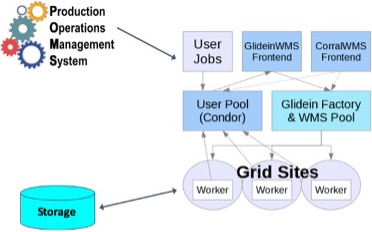
\includegraphics[width=\textwidth]{graphics/Workflow/POMSWorkflow.jpg}
\caption{Overview of the current DUNE Production workflow setup used also by the \dword{proto} detectors for data reconstruction and simulation. Production group members interact with \dword{poms} to submit jobs, which uses the Jobsub tool to submit jobs to a HTCondor scheduler. GlideinWMS provisions worker node resources and jobs match to the available worker node slots. DUNE jobs interact with storage elements  at Fermilab and other sites both for input copy (or streaming for most production workflows) and output copyback.}
\label{fig:workflowPOMS}       % Give a unique label
\end{figure*}

Choosing a Glidein-based system at this stage of the experiment had several advantages. DUNE was able to quickly leverage the existing FIFE~\cite{herner2019advances} toolset, including \dword{poms} and Jobsub, negating the
need for significant effort from the experiment in getting jobs running quickly (let alone in designing a completely new system). Since the system is in use by other neutrino experiments at Fermilab, it is easy for new DUNE collaboration members coming from these experiments to 
begin submitting jobs quickly as they are working with a familiar system. The DUNE Production workflows were also able to leverage the existing infrastructure support teams in place to server other collaborations and consortia such as 
CMS and OSG. Finally, as GlideinWMS is widely used in HEP, setting up new sites becomes extremely straightforward, especially if the site is already supporting another experiment that uses GlideinWMS. Our integration times for new 
DUNE sites are typically less than one week and successful production jobs immediately after opening up the site are now the rule rather than the exception. This ease of setup has been a key enabler of DUNE's international expansion. From January to November 2019, sites outside the United States delivered approximately 49\%\ of the total DUNE Production wall hours as shown in Figure~\ref{fig-country}. International sites regularly run the full suite of DUNE jobs, including ProtoDUNE data reconstruction and user analysis. % DUNE is also considering the creation of a global GlideinWMS pool similar to the CMS Global Pool~\cite{cmsgp,cmsgp2}, which would enable multiple institutions to set up their own submission hosts if they desired to do so.

\begin{figure*}[htb]
\centering
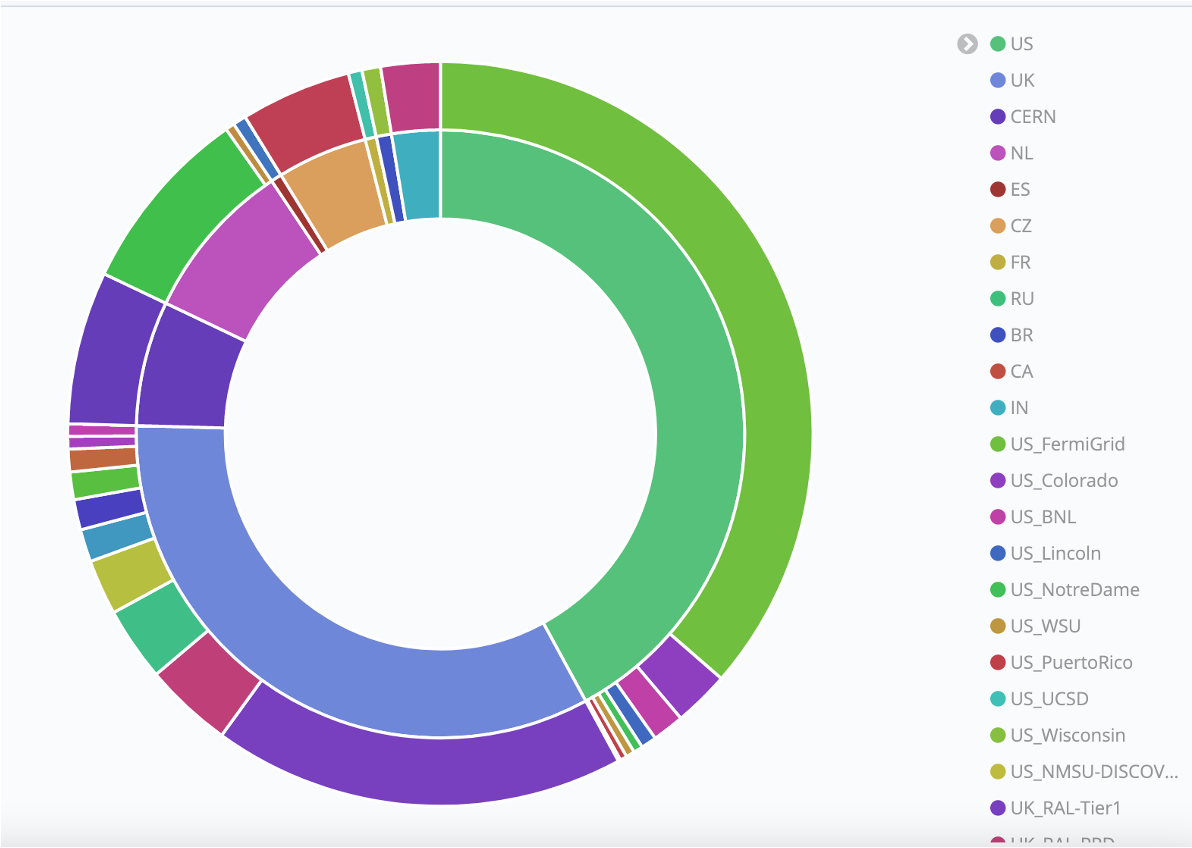
\includegraphics[width=\textwidth]{graphics/Workflow/August2021.png}
\caption{Wall time-weighted distribution of successful DUNE Production jobs for August 2021. Inner ring: distribution by country. Outer ring: distribution by site. Sites outside the United States delivered 60\%\ of the total wall hours for the jobs shown here.}
\label{fig-country}       % Give a unique label
\end{figure*}

\subsection{DUNE software, input data distribution, and output file handling}
\label{subsec:io}
DUNE builds its software suite for  Scientific Linux. Since October 2019 DUNE jobs will automatically run inside a Singularity container at supported sites via a GlideinWMS mechanism that requires no user knowledge of Singularity other than specifying the desired image, reducing the possibility of errors and guaranteeing a homogeneous environment across all sites.

For its file catalog, DUNE uses Fermilab's \dword{sam} system~\cite{Illingworth:2014mba}, which handles input file selection and delivery for each job, and has been successfully used by numerous HEP experiments for well over a decade. As described in Chapter \ref{ch:datamgmt},  in future we expect Rucio~\cite{Barisits:2019fyl} will  take over most of these functions. Production jobs typically stream input data files via \dword{xrootd}, though in some cases they will copy a file to the worker node and directly read the local copy. The data source can be any storage system reachable from the worker
node and to which DUNE has access. This is most often Fermilab dCache, but CERN EOS and other storage elements in Europe are also used (jobs run at CERN would get their inputs from CERN EOS, for example). Several DUNE workflows require one or more auxiliary input files (i.e. not detector data) such as calibration files, neutrino flux information, and other inputs necessary for analysis for MC generation. Some simulation workflows randomly
choose several such input files for each job from a much larger set, so the file overlap between jobs is small. Additionally the files are typically tens of MB in size. These two attributes make these files poor candidates for placement in a standard \dword{cvmfs} repository. For such files we store them in a \dword{stashcache}~\cite{bib:stashcache} repository,
accessible in a POSIX-like fashion though a \dword{cvmfs} overlay. With this method there is still some level of shared caching on a worker node, but as files need to be copied in from the source (Fermilab \dword{dcache}), it happens in a transparent way, meaning the user can simply access the files via a CVMFS path in the dune.osgstorage.org repository.

For output file handling nearly all workflows currently copy their outputs to Fermilab \dword{dcache}, with a small minority (ProtoDUNE-DP jobs) also copying to a storage element at IN2P3 in France. We use Rucio to manage file replication
to other sites. In the future DUNE will likely move to a more distributed copyback model: at sites with local storage, a job can simply copy its output to a local location, and then we can use Rucio for replication as is already done, rather than requiring everything first go through Fermilab.

There is an exception for workflows run at NERSC; we read input auxiliary files from and copy output files out
to Cori's global scratch filesystem. For job outputs, a separate process performs bulk transfer back to Fermilab from one of NERSC's dedicated data transfer nodes. We expect that workflows on other future HPC platforms
will follow a similar approach, especially at places without external connectivity on the worker nodes.


\section{Workflow Proposal} 
\subsection{Request lifecycle}
\label{sec:flow:lifecycle}

The central concept of the workflow system is a request, which describes how some data processing activity is to be carried out. Requests are submitted by users (which may include members of a central production team) to the Workflow Database described below. Each request can be in one of several states, which it progresses through. For example, draft > submitted > approved > running > paused > running > checking > completed > archived. Human intervention is needed for some transitions: for example, from submitted to approved. Requests also have types and priorities. For example, simulation or user analysis; high or low.

As part of its definition, a request may include one or more stages which can apply a sequence of processing steps to the files the request uses or generates. Each stage specifies a bootstrap script used by generic jobs to run the relevant applications, requirements on the worker nodes eligible to run that stage (for example memory), and the maximum number of input files to be issued to a generic job executing that stage.

The definition of a request will include an MQL query which can be submitted to MetaCat to generate a list of files to be processed in the first stage. This list of files is cached in the central Workflow Database, associated with the first stage of that request. All these files are set to the unallocated state. 

The request definition is an input to the Data Management placement agent which transfers replicas of files to suitable sites, based on the description of the request and knowledge of site features. The location of the replicas of the files is also included in the database, cached from RUCIO. 

Once the various agents have finished building the request, it can move to the running state and the bootstrap script associated with the first stage will begin to be executed at sites to process files.


\begin{dunefigure}
[Workflow and data management architecture diagram]
{fig:workflow} 
{Workflow and data management architecture diagram.}
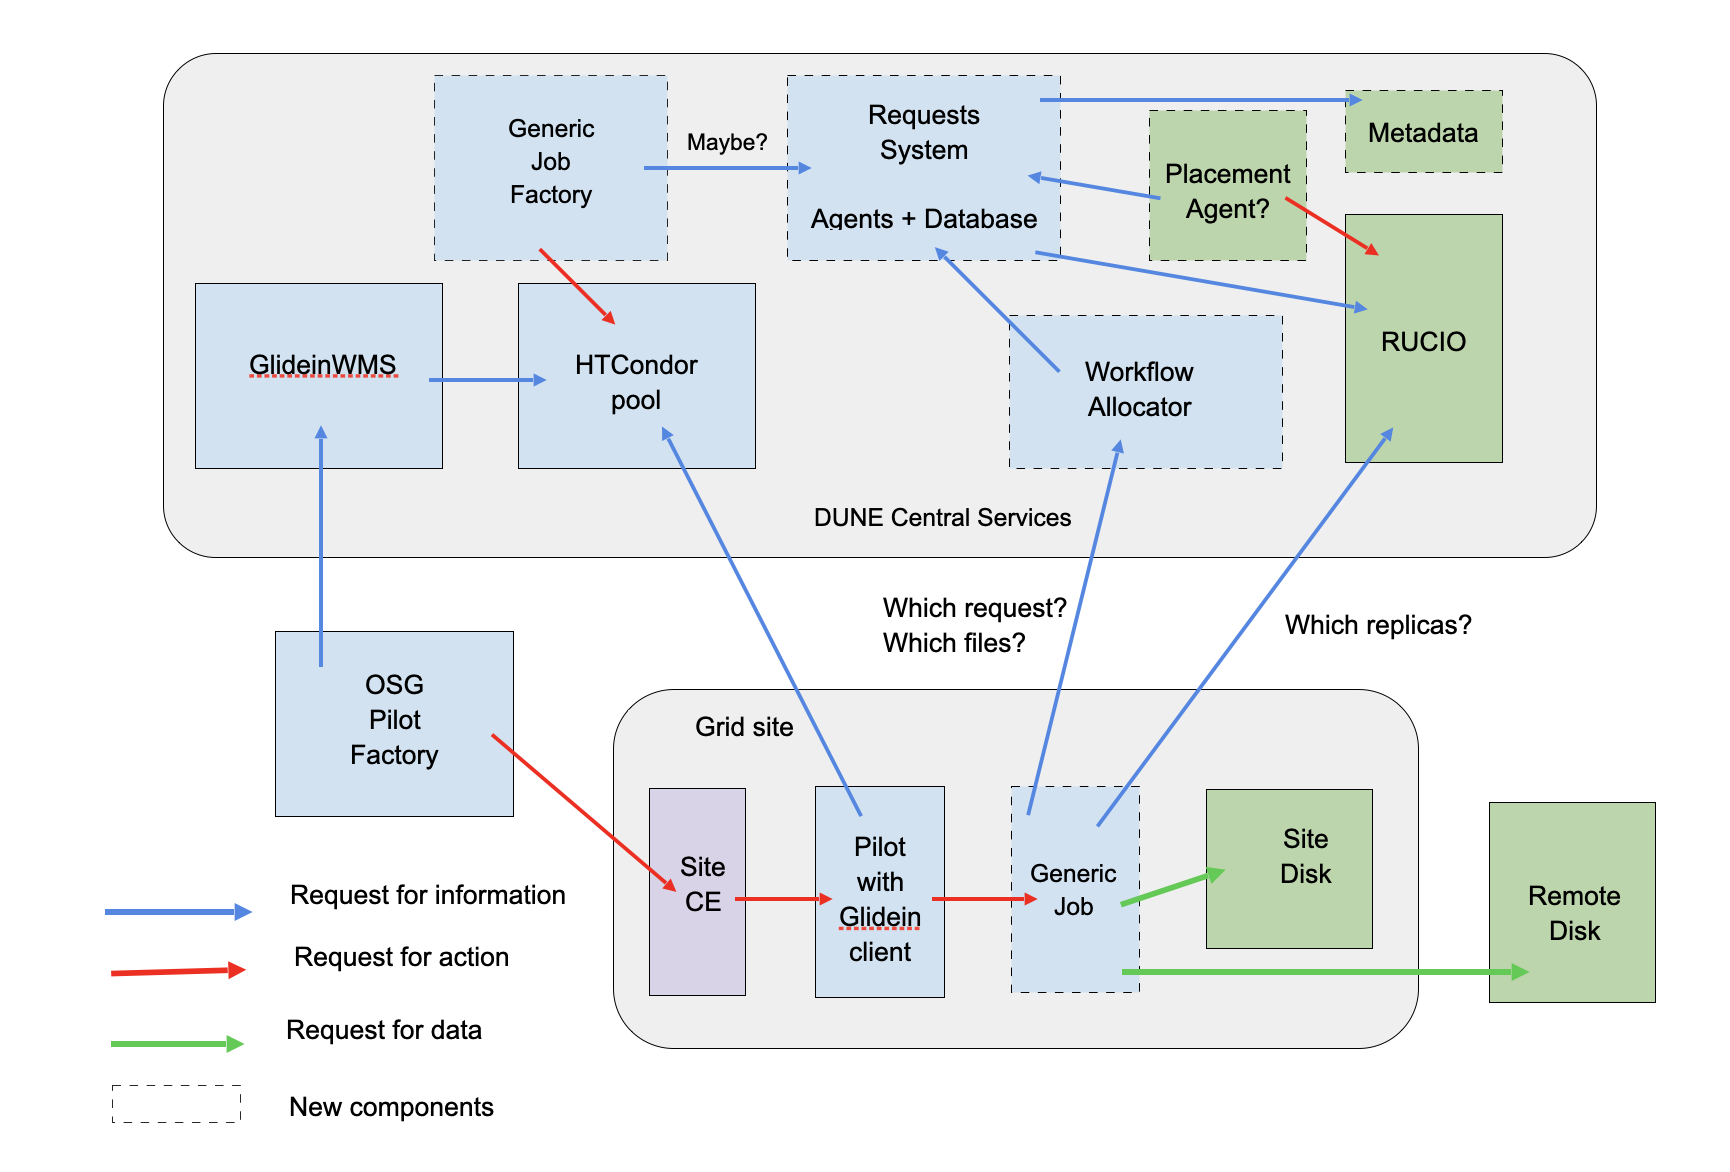
\includegraphics[height=8cm]{graphics/Workflow/wfs.png}
\end{dunefigure}\todo{Get better figure}

\section{Grid workload systems}
\label{sec:flow:grid}

The workflow system makes use of the existing global grid infrastructures to deliver jobs for execution on worker nodes at sites. This allows us to operate alongside other experiments in the Worldwide LHC Computing Grid without placing special requirements on sites.

FNAL operates a global HTCondor pool for DUNE which makes use of the existing OSG Pilot Factory service and HEPCloud to provision execution slots at sites. By using these existing systems we are able to use computing capacity presented with ARC CE or HTCondor CE grid interfaces, or on cloud and High Throughput Computing services supported by HEPCloud.

\section{Generic job factory}
\label{sec:flow:factory}

The Generic Job Factory agent creates and submits HTCondor jobs which are each assigned to a single execution site. It will use a mixture of matching successes, site limits from DUNE CRIC, and prioritization of sites to determine how many generic jobs to submit and have waiting at each site. It may also use inspection of the central workflow database to estimate whether more generic jobs should be submitted for a particular site. For ordinary jobs, the job factory must be able to prioritise use of pledged academic and lab sites over commercial cloud sites and specialised sites like NERSC, which are managed by HEPCloud, to allow those services to be used for specialised workflows. Inspection of files waiting to be allocated in the database may be more appropriate for HEPCloud managed sites, so that work requiring their features may be satisfied.

Once a generic job lands on a worker node, it contacts the Workflow Allocator described later which determines which unallocated files from one stage best match that worker node.

\section{Workflow Database}
\label{sec:flow:wfdb}

The central Workflow Database stores definitions of requests and their stages, and cached information about files, replicas, sites, and storage services. Together all this information is used by queries to determine what work to carry out where. It is implemented as an SQL relational database.

\subsection{Information Collector}
\label{sec:flow:collector}

The Information Collector agent will run periodically to obtain a list of eligible sites and storage services from CRIC and other information sources, including any downtime notifications. 

\subsection{Request Builder}
\label{sec:flow:builder}

The Request Builder agent will use the input dataset definition in a request to construct a list of input files for the first stage of that request. Typically this involves making queries to MetaCat to obtain a list of files in the given dataset. This list is cached within the Workflow Database so it can be used as part of the SQL queries. As the files are identified, the location of their replicas are also obtained and cached from RUCIO. Again, this allows the proximity of replicas of unprocessed files to be used in deciding what work a job should do.

\subsection{Archiver}
\label{sec:flow:archiver}

The Archiver agent will have responsibility for removing information about requests, stage, files, and replicas once they are no longer needed, archiving whatever is needed for future reference to long term storage. It is intended that important information about how and where files were processed will be stored in the MetaCat database by the generic jobs themselves, but some higher level information about the operation of the workflow system and the processing of requests will be saved by the Archiver.

\section{Workflow Allocator}
\label{sec:flow:allocator}

Once a generic job arrives at a worker node, it contacts the Workflow Allocator service which determines which unallocated file from one stage best matches that worker node. This matching includes the characteristics of the worker node job slot (memory, time limit etc), and whether the site is eligible to access a replica of that data file. Replicas are prioritised based on whether the worker node and replica are at the same site, ``nearby'', or elsewhere but still eligible. 

A list of suitable input files from the same, matching stage is returned to the generic job, along with the bootstrap script to run. Each input file successfully processed by the application is reported to the Workflow Allocator so that the input file’s status can be updated from Allocated to Processed. Unprocessed input files are returned to the unallocated state for processing in another job. 

If the stage is not the final stage for that request, each output data file is also inserted into the list of files associated with the next stage for that request, in the unallocated state. 

\section{User commands}
\label{sec:flow:commands}

Command line tools are provided to operators and users to allow queries of Workflow Database contents and the creation of requests. These tools are envisaged to be of most use during testing of new workflows and for short workflows during analysis. 

\section{Workflow Dashboard}
\label{sec:flow:dashboard}

The same functionality as the command line tools outlined above will be provided by a Workflow Dashboard web interface. This will allow more sophisticated searches in the Workflow Database to monitor the progress of running requests, and allow members of the operations team to examine the state of the system at the level of individual files and replicas which are due to be processed, or have recently been processed to enable debugging of problems with sites or workflow definitions.

The Workflow Dashboard is also intended to be used for all large scale productions, and will allow submitters to draft request definitions, circulate their proposal with colleagues for checking, before submitting them to any formal approval and checking procedure. The lifecycle of a workflow request accommodates manual approval and prioritization of large requests while smaller requests can be approved automatically according to a pre set limits. A library of bootstrap script templates and requests will be provided as part of the dashboard to help users make sensible choices for common types of workflow.

\end{document}